\subsection{Linking the Past to Present}

While a recent wave of scholarship systematically and quantitatively documents the impact of historical events on contemporary political and economic phenonemon, one of the main shortcomings of this literature is that the causal mechanisms that attribute to the persistence of historical events or institutions largely remain in a ``black box" \citep{ImaiEtAl2011,AcharyaBlackwellSen2016}. Given that the authors estimate effects that persist over hundreds of years, this concern is especially acute for understanding how historical conflict shapes contemporary conflict and cooperation. In their paper, the authors lay out several paths through which the effects of pre-colonial conflict might persist until today and, to their credit, they test several of the observable implications. The primary empirical challenge, however, is to systematically analyze the degree to which the effects of pre-colonial conflict in Africa flow through certain hypothesized mechanisms. In the previous section, we argued that automated approaches suggest that some of these interactions are especially useful in explaining variation in modern outcomes. In this section, we address a similar conceptual concern - how to identify the key mechanisms - by estimating the Average Controlled Direct Effect (ACDE) of historical conflict on contemporary outcomes as a strategy to rule out certain causal pathways that explain the persistence of pre-colonial conflict on African political economy.

Before laying out the assumptions needed to identify the ACDE of pre-colonial conflict as well the procedure to consistently estimate this quantity of interest, we first present \citet{BesleyRQ2014}'s preferred causal mechanisms in greater detail. In general, \citet{BesleyRQ2014} argue that the presence of historical conflict at both the national and subnational level enervates political and economic development. Particularly, the authors highlight two mechanisms:

\begin{displayquote}
...conflicts can affect the evolution of subsequent economic, political, and social outcomes which have a bearing on contemporary conflict. For example, historical conflicts could promote distrust among social groups which affect attitudes and identities. They could also have an economic legacy, making regions poorer and could also influence the choice of political institutions. \citep[pg. 321]{BesleyRQ2014}.
\end{displayquote} 

While the authors present a number of empirical tests for these mechanisms in Tables 4 and 5 in their paper, there are a number of problems in the approach that they take. First when the authors estimate the effect historical conflict on contemporary levels of trust, ethnic identity, and national identity, they include a number of post-treatment confounders that both could be biasing their estimates as well as obscuring the actual mechanisms driving their results. For example, the historical conflict may shape contemporary social identities, but this effect only runs through the ways in which adverse economic development or political institutions shape social identity. By conditioning on variables such as contemporary levels of conflict and economic development, the authors leave themselves open to the possibility of post-treatment bias in estimating the effect of historical conflict on identity and trust. In essence, contemporary economic and development and conflict are themselves potential mediators for the effect of pre-colonial conflict on identity politics.

Second, the authors attempt to make empirical claims about the subnational effects of historical conflict on contemporary conflict and development. Again, the authors condition on a post-treatment confounder--the grid-level population density in 1990--which itself is also likely to be a product of historical conflict since population density is a proxy for development in agricultural economies. Since simply conditioning on post-treatment variables is not enough to determine the direct effect of a variable, it is unclear as to the magnitude of the direct effect of pre-colonial conflict on contemporary conflict and development. In the rest of this section, we present the identifying assumptions needed to estimate the ACDE of pre-colonial conflict in addition to estimating this quantity of interest using Sequential-G estimation \citep{JoffeGreene2009,Vansteelandt2009,AcharyaBlackwellSen2016}. 


\subsection{Estimating the Average Controlled Direct Effect}

Intuitively, the ACDE is the direct effect of the treatment variable of interest (historical conflict) holding some mediator (economic development for example) fixed at a certain value. The advantage of this quantity of interest is that it represents the effect of historical conflict independent of a particular causal channel. As \citet{AcharyaBlackwellSen2016} point out, this can help researchers rule out whether certain causal mechanisms drive a certain set of results, which can help adjudicate between competing theories of politics. In this case, the authors are interested in two sets of ACDEs. First, the authors want to be able to assess whether pre-colonial conflict in Africa has a direct effect on identity and trust net of its effect on economic development and conflict. Second, the authors aim to make an empirical claim that historical conflict shapes contemporary economic development and politics independent of its demographic consequences on population density.

To estimate these sets of ACDEs, we need to make certain assumptions about the data-generating process. Primarily, we must make an assumption of \emph{sequential ignorability} \citet{Robins1997,AcharyaBlackwellSen2016}. That is, historical conflict is plausibly exogenous given a set of background covariates such as latitude, longitude, historic population density, etc. and that the proposed mechanism is plausibly exogenous conditional on both historical conflict and the background covariates. Most notably, \citet{ImaiEtAl2011} also rely on this assumption to assess the Average \emph{Natural} Direct Effect (ANDE) and the Average Natural Indirect Effect {ANIE}. Nonparametrically identifying these estimands relies on a further assumption of no intermediate confounders, which in most observational (and even experimental studies) is unlikely to hold. Thus, the ACDE can be identified under a weaker set of assumptions. The tradeoff, however, is that the ANDE and ANIE might be more suited to assessing competing mechanisms against each other. 

For this paper, we utilize the Sequential-G estimation strategy discussed in \citet{AcharyaBlackwellSen2016} and developed by \citet{JoffeGreene2009,Vansteelandt2009}. The basic intuition behind this estimation procedure is that we first estimate a regression including both historical conflict and the potential mediators (economic development and civil conflict) on the right-hand side. This is what \citet{BesleyRQ2014} do to assess the direct effect of pre-colonial conflict. The problem with only running this regression is that it induces bias of an unknown sign and magnitude \citep{AcharyaBlackwellSen2016}. Instead, we take fitted values from that initial regression and ``demediate" the outcome netting out the effects of these mediators on the outcome of interest and re-run a regression of the ``demediated" variable on historical conflict. This approach, allows us to estimate the ACDE of historical conflict on the outcome of interest consistently. 

To assess the direct effect of pre-colonial conflict on social identity, contemporary development, and civil conflict, we reanalyze the data used to produce the results for Tables 4 and 5 in the authors' main paper. First, we assess the direct effect of pre-colonial conflict on strength of ethnic identity, national identity, and intergroup trust by estimating the following sets of equations:

\begin{equation}
Y_i = \alpha + \beta \text{Historical Conflict}_i + \lambda \text{Log(GDP per Capita, 1960)}_i + \gamma \text{Civil War Incidence} + \phi X_i + \epsilon_i
\end{equation}

\begin{equation}
Y_i - \widehat{\lambda} \text{Log(GDP per Capita, 1960)}_i - \widehat{\gamma} \text{Civil War Incidence}= \alpha + \beta \text{Historical Conflict}_i + \phi X_i + \eta_i
\end{equation}

$Y_i$ represents the outcome of interest indexed by each respondent $i$. In this case, it is either whether the Afrobarometer respondent identifies more with his or her own ethnicity over other possible identities, identifies more with his or her national identity, and whether the respondent trusts members of other ethnic groups. The main coefficient of interest is $\beta$, which represents the ACDE of historical conflict. The coefficients $\lambda$ and $\gamma$ represent the effects of the mediators contemporary development and civil conflict respectively. Finally, the matrix $X_i$ represents the set of pre-treatment controls and fixed effects while $\epsilon_i$ and $\eta_i$ represent Gaussian error terms. 

We estimate a similar set of equations in our reanalysis of Table 5 from the original paper, which investigates the direct effect of historical conflict on subnational economic and political development at the grid-cell level. Thus, we estimate the following set of equations:

\begin{equation}
Y_g = \alpha + \beta \text{Historical Conflict}_g + \kappa \text{Log(Population Density, 1990)}_g + \phi X_g + \epsilon_g
\end{equation}

\begin{equation}
Y_g - \widehat{\kappa} \text{Log(Population Density, 1990)}_g = \alpha + \beta \text{Historical Conflict}_g + \phi X_g + \eta_g
\end{equation}

For these estimating equations, $Y_g$ represents the incidence of conflict or the light density (proxy for development) at the grid-cell level $g$. $X_i$ represents the authors' specified set of pre-treatment control variables. Finally, both equations have Gaussian error terms $\epsilon_g$ and $\eta_g$ respectively. 

\subsection{Results} \label{acderesults}

\begin{figure}
\begin{center}
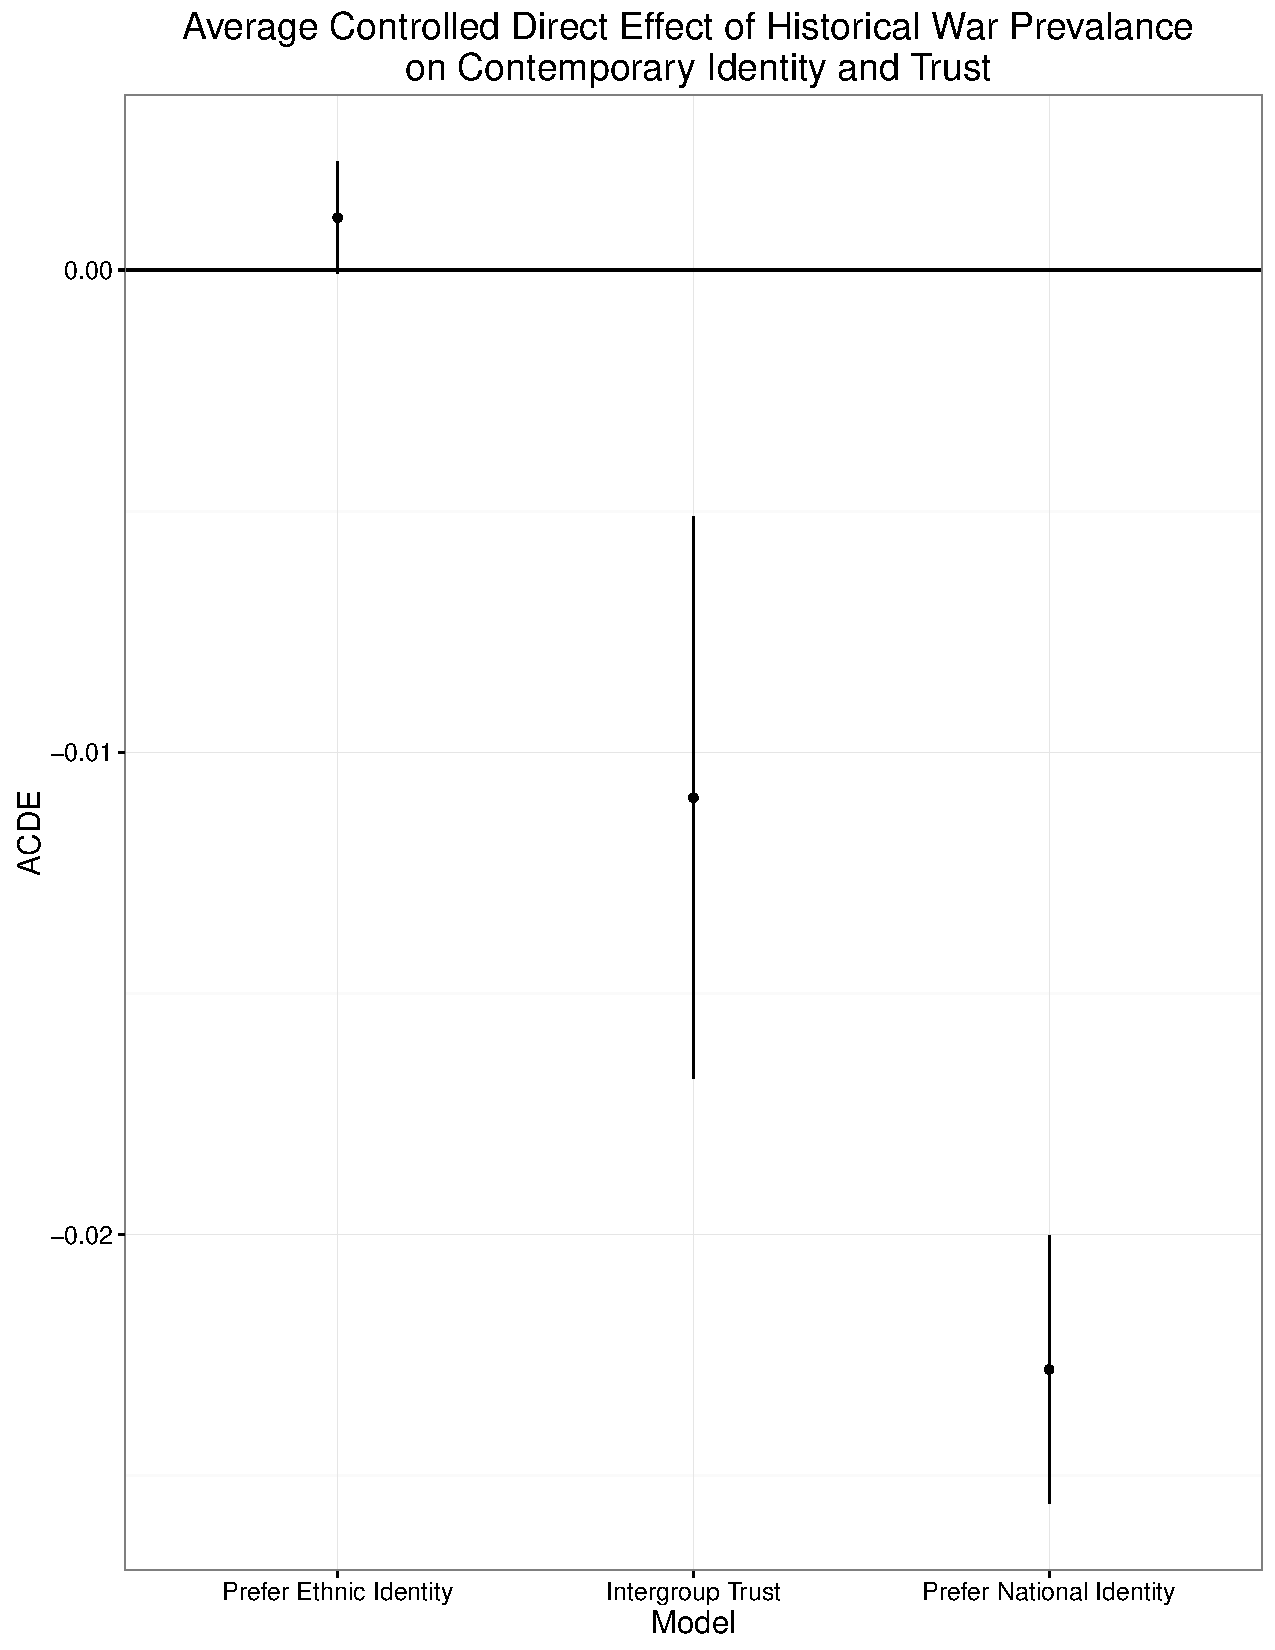
\includegraphics[scale=0.3]{Figures/acde_trust}
\caption{ACDE of historical conflict in Africa on ethnic identity, national identity, and intergroup trust netting out the effect of economic development in 1960. All models are estimated using the Sequential-G procedure described in \citet{AcharyaBlackwellSen2016}. Models include the original pre-treatment control variables.}
\label{fig:acdetrust}
\end{center}
\end{figure}


\begin{figure}
\begin{center}
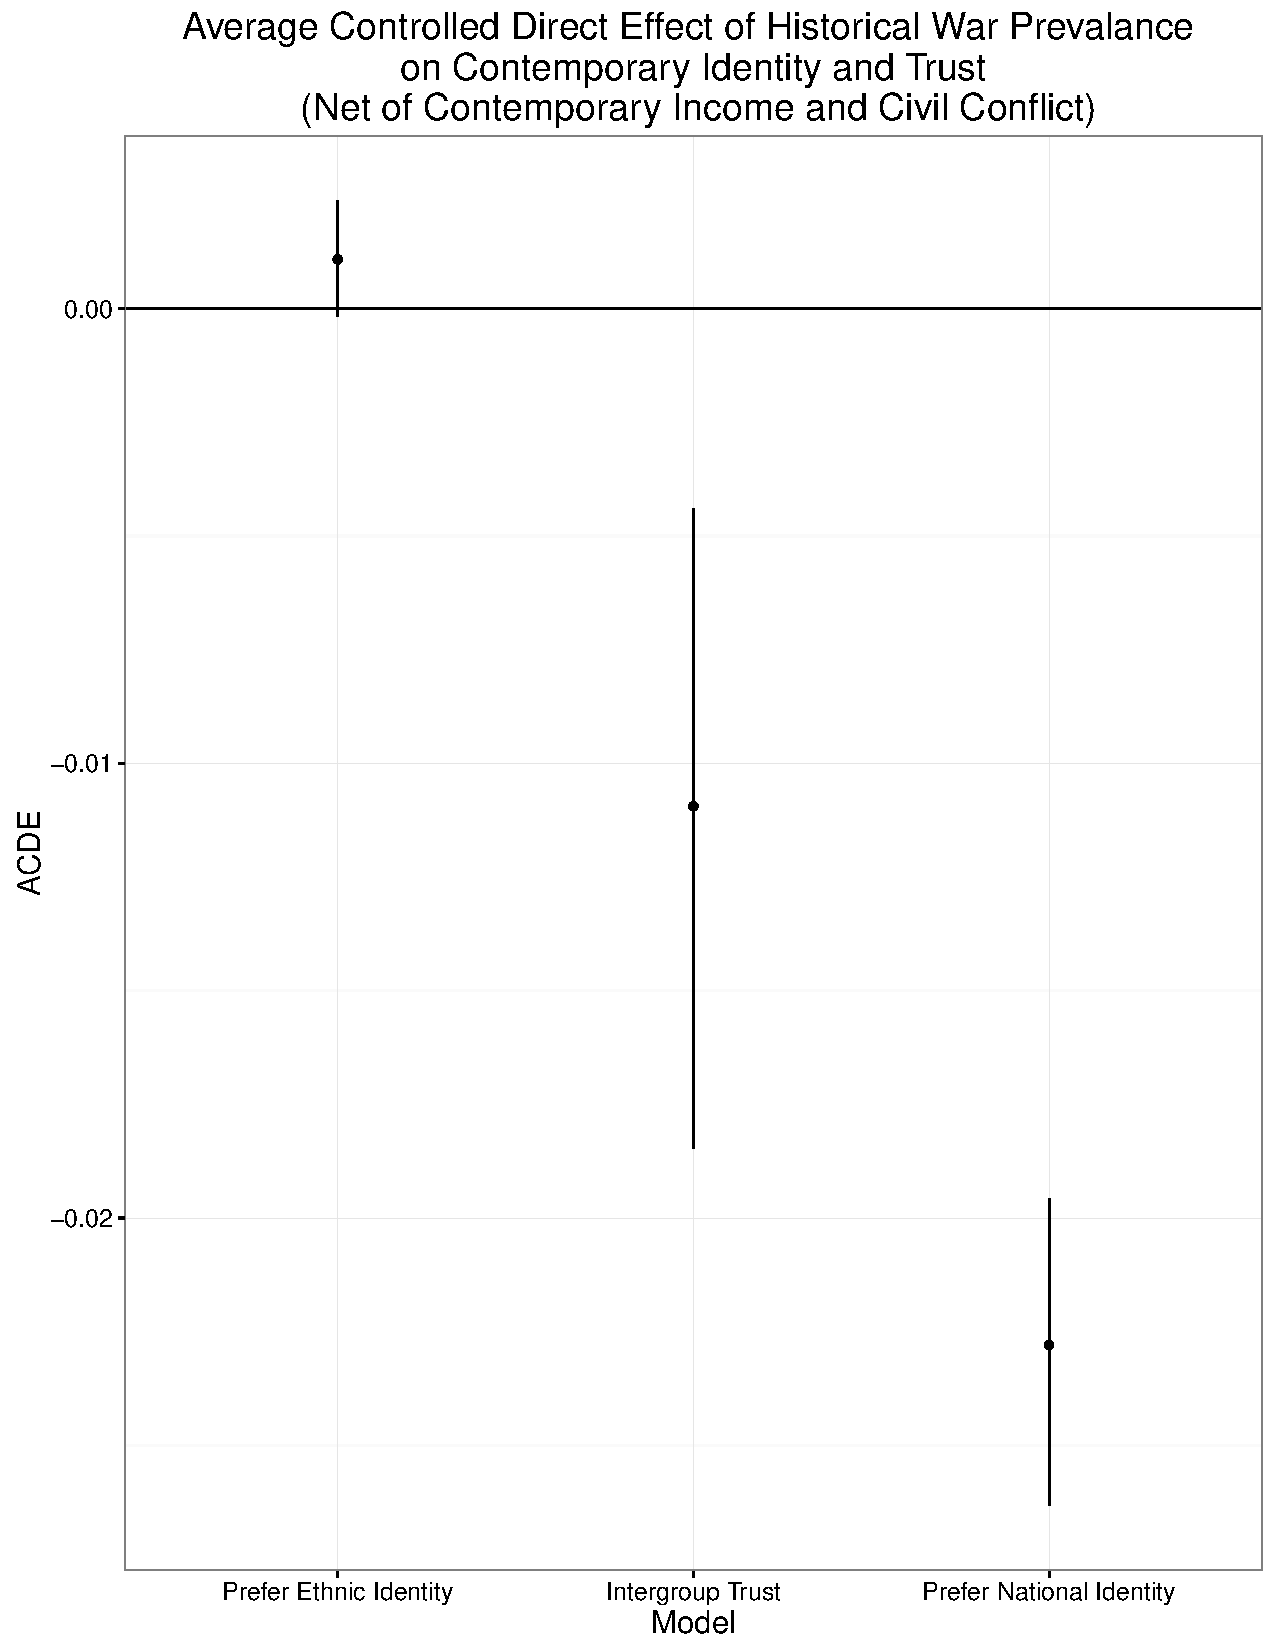
\includegraphics[scale=0.5]{Figures/acde_war_trust}
\caption{ACDE of historical conflict in Africa on ethnic identity, national identity, and intergroup trust netting out the effect of economic development in 1960. All models are estimated using the Sequential-G procedure described in \citet{AcharyaBlackwellSen2016}. Models include the original pre-treatment control variables.}
\label{fig:acdewartrust}
\end{center}
\end{figure}

In the first set of results shown in Figure \ref{fig:acdetrust} we estimate the ACDE of historical conflict on ethnic identity, national identity, and intergroup trust and only demediate the outcome variables by the log of GDP per capita in 1960. We find that historical conflict seems to have a direct effect on social identity with the magnitudes of the effect in the same signs and magnitude as the specifications used in Table 4 of \citet{BesleyRQ2014}. On average, a one unit increase in the ACDE of conflict seems to increase the salience of the respondent's ethnic identity by about 0.1 percentage points with the effect being just marginally insignificant at the $p<0.05$ level, decrease the degree to which the respondent trusts individuals from other ethnic groups by about 1 percentage point, and decrease the degree to which the respondent identifies with his or her national identity by just over 2 percentage points. We find a similar pattern of results when we net out the effect of both contemporary development and contemporary civil conflict on social identity as shown in Figure \ref{fig:acdewartrust}. 

These results speak to the authors' theory in a number of ways. It seems that the prevalence of precolonial conflict seems to operate independently of these economic and political channels hypothesized by the authors. Instead, the evidence suggests that pre-colonial conflict shapes social identity through cultural or institutional channels. These results, then, motivate further inquiry how the prevalence of pre-colonial conflict might shape the formation, amalgamation, or dissolution of various ethnic groups. These results complement the LASSO analysis in section 2, which demonstrated that the incidence of pre-colonial conflict explained important elements of the cross-country variation, and that particular interactions - for example, through exposure to the slave trade - appeared to play a central role in explaining variation in modern social attitudes. 

In the next part of the original paper, \citet{BesleyRQ2014} investigate the effects of pre-colonial conflict on \emph{subnational} conflict and development. To do so, the authors utilize grid-cell level data on conflict and night light density (a commonly used proxy for development) as the dependent variables to be explained. Figure \ref{fig:acdegrid} provides evidence that pre-colonial conflict does have a direct effect on contemporary subnational conflict incidence net of the effect of conflict on population density in 1990 (a proxy for urbanization and development). This general finding is consistent with the authors' original findings on conflict in Table 5 of the main paper. Contrary to \citet{BesleyRQ2014}, however, we find that pre-colonial conflict does not have a direct effect on contemporary levels of economic development as proxied by night light density in 2007 independent of its effect on subnational urbanization at conventional levels of statistical significance. 

Theoretically, the results from this set of tests suggest two main theoretical contributions. First, it seems that historical conflict at the subnational level seems to operate independently of its consequences on demographics. As a result, it could be the case that historical conflict shapes subnational politics through some sort of cultural or local institutional mechanism that operates independently of demographics and economic development. This evidence is consistent with our findings from the previous empirical test where we showed that the effect of pre-colonial conflict seems to operate independently of its effect on national economic development. Next, we find that subnational, historical conflict does not shape subnational economic development independent of its effect on demographics and urbanization. These results raise a puzzling tension for the authors' original theory that states that conflict historical conflict shapes contemporary development primarily through a mechanism where conflict begets conflict leaving areas in a sort of a conflict trap. Thus, the subnational results from this Sequential-G estimation strategy indicate that the channels through which pre-colonial conflict shapes contemporary economic development is quite different from the process through which pre-colonial conflict shapes contemporary conflict. 

\begin{figure}
\begin{center}
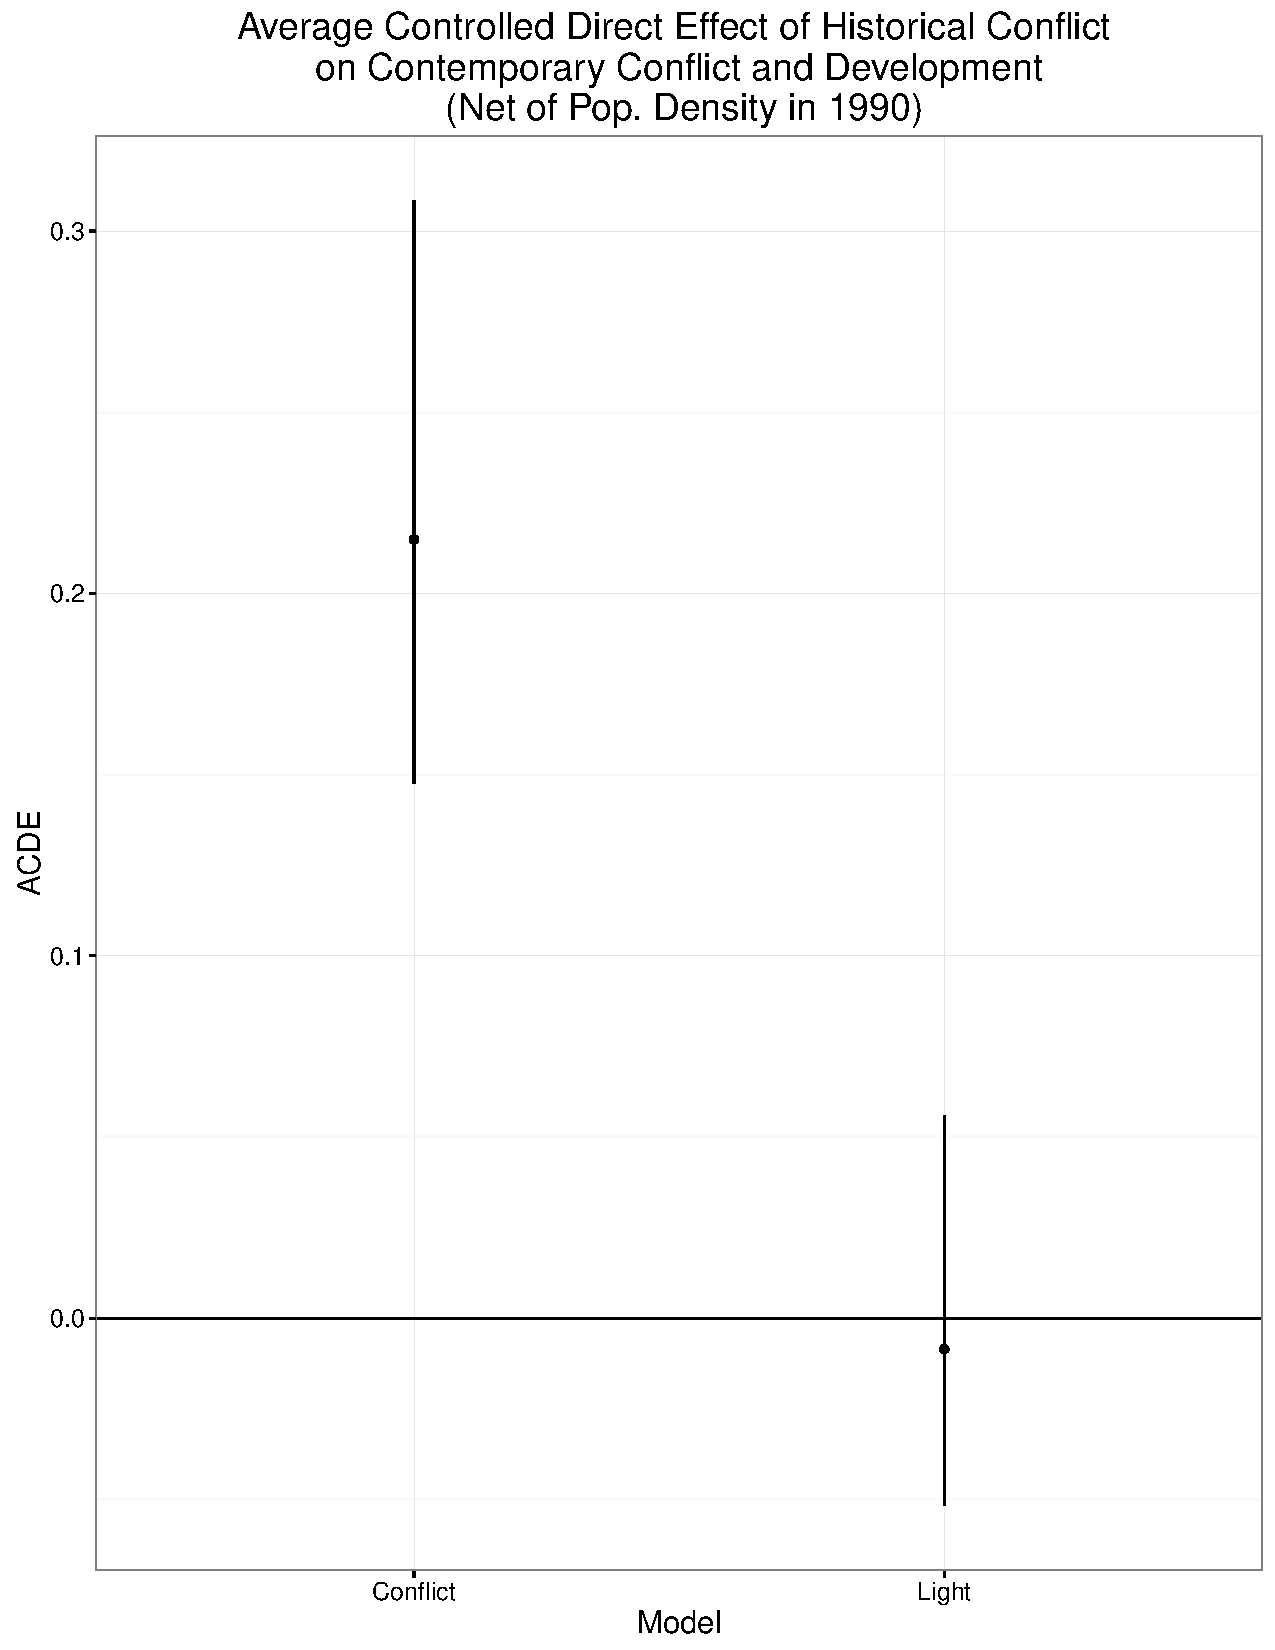
\includegraphics[scale=0.5]{Figures/acde_grid}
\caption{ACDE of historical conflict in Africa on contemporary conflict and light density at the grid-cell level netting out the effect of population density in 1990. All models are estimated using the Sequential-G procedure described in \citet{AcharyaBlackwellSen2016}. Models include the original pre-treatment control variables.}
\label{fig:acdegrid}
\end{center}
\end{figure}

